\documentclass[11pt]{ctexart}
\usepackage[margin=2.6cm]{geometry}
\usepackage{amsmath,amssymb,amsthm}
\usepackage{booktabs,array}
\usepackage{tikz,xcolor}
\usepackage{xcolor}
\usepackage{mdframed}

% 定义 Markdown 风格的引用块环境
\newmdenv[
  topline=false,        % 不显示顶线
  rightline=false,      % 不显示右线
  bottomline=false,     % 不显示底线
  leftline=true,        % 显示左线
  linewidth=3pt,        % 左线宽度
  linecolor=gray!50,    % 左线颜色
  backgroundcolor=gray!10, % 背景色
  innerleftmargin=10pt, % 文本与左线的距离
  innerrightmargin=10pt, % 右侧内边距
  innertopmargin=8pt,   % 顶部内边距
  innerbottommargin=8pt,% 底部内边距
  skipabove=8pt,        % 与上方文本的间距
  skipbelow=8pt         % 与下方文本的间距
]{markdownquote}

% 将默认的 quote 环境重定义为 markdownquote
\renewenvironment{quote}{\begin{markdownquote}}{\end{markdownquote}}

\definecolor{figA}{RGB}{214,231,247}
\definecolor{figB}{RGB}{247,224,214}
\definecolor{figC}{RGB}{219,242,222}
\definecolor{figD}{RGB}{244,238,211}
\definecolor{figE}{RGB}{233,220,244}
\definecolor{figF}{RGB}{215,240,240}
\tikzset{ked/.style={line width=0.75pt},
         gone/.style={red!75!black, densely dotted, line width=1.05pt}}

\newtheorem{theorem}{定理}[section]
\newtheorem{lemma}[theorem]{引理}
\newtheorem{proposition}[theorem]{命题}
\newtheorem{corollary}[theorem]{系}
\newtheorem{conjecture}[theorem]{猜想}
\theoremstyle{definition}
\newtheorem{remark}[theorem]{注}
\newtheorem{fact}[theorem]{计算事实}
\renewcommand{\proofname}{证明}

\newcommand{\ceil}[1]{\left\lceil #1 \right\rceil}
\newcommand{\floor}[1]{\left\lfloor #1 \right\rfloor}

\title{网格图中的矩形消边问题：$S(4,m)$ 至 $S(8,m)$ 的精确值\\与一个奇偶障碍定理}
\author{（作者待填）}
\date{2026 年 7 月}

\begin{document}
\maketitle

\begin{abstract}
本文研究如下问题：在一个有 $n$ 行、$m$ 列单位小方格的网格图中，最少删除多少条边，才能保证剩下的图中不再出现任何由网格线组成的矩形边界？把这个最小删除数记为 $S(n,m)$。Niu 与 Tang \cite{NT25} 已经确定了 $n\le 3$ 时的精确值，并对 $S(5,m)$ 给出了只相差 $1$ 的上下界。本文进一步完全确定了 $n=4,5,6,7,8$ 时所有 $m$ 对应的 $S(n,m)$。

最特别的结果是
\[
S(4,m)=\ceil{30m/11}\qquad(m\ge2).
\]
这说明高度为 $4$ 的网格有一个特殊的渐近删除密度 $30/11$，它严格大于通常由三格骨牌铺砌所给出的欧拉型下界 $8/3$。本文还证明，除高度 $4$ 外，所有 $n\ge5$ 的高度都满足
\[
\lim_{m\to\infty}\frac{S(n,m)}m=\frac{2n}{3}.
\]

本文的核心新工具是一个纯组合的\textbf{奇偶障碍定理}：当 $nm\equiv1\pmod3$ 时，如果欧拉型下界能够取等号，即
$S(n,m)=\ceil{2nm/3}$，那么 $n$ 和 $m$ 必须都是偶数。这个定理给出了三族重要下界的人工证明：$S(5,3k+2)$、$S(7,3k+1)$ 和 $S(8,6t+5)$ 都比欧拉型下界至少大 $1$。它也解释了为什么 Golomb 的某类构造能够用于 $2^k\times2^k$ 网格。

此外，本文通过一个带有接口条件的分层拼接引理，补充并推广了 \cite{NT25} 的定理 3，去掉了原结果中 $m\ge n\ge8$ 的限制。对于特殊高度 $4$，本文还给出一个可以逐项独立检查的势函数表，用它证明
$S(4,m)\ge30m/11$。文中所有依赖计算的结论，都说明了有限状态如何产生、需要检查哪些数据，以及如何通过独立程序复核。
\end{abstract}

\section{引言}

先说明本文研究的对象。一个 $n\times m$ 网格图由 $(n+1)(m+1)$ 个格点组成：相邻格点之间用一条单位边连接。因此，它有 $(n+1)(m+1)$ 个顶点，以及 $2nm+n+m$ 条边。这里的 $n\times m$ 指网格中有 $n$ 行、$m$ 列单位小方格。

我们所说的\emph{矩形}，不只包括一个单位小方格，也包括由若干行、若干列小方格拼成的任意长方形。它的四条边都沿着网格线，并且四条边组成一个闭合回路。我们把这个回路称为\emph{矩形轮廓}。例如，取两条不同的水平网格线和两条不同的竖直网格线，它们围成的边界就是一个矩形轮廓。

现在允许我们从网格图中删除边，但不删除顶点。若删除边集 $A$ 后，剩余图中已经找不到任何矩形轮廓，就称 $A$ 是一个\emph{矩形消去集}。本文研究的量
\[
S(n,m)=\min\{|A|: A\text{ 是一个矩形消去集}\}
\]
就是完成这件事至少需要删除多少条边。换句话说，我们希望用尽可能少的删除操作，破坏网格图中的每一个矩形边界。

这个问题由 Niu--Tang \cite{NT25} 系统研究。他们已经得到
\[
S(1,m)=m,\qquad
S(2,m)=\ceil{3m/2},\qquad
S(3,m)=2m+1,
\]
并证明了适用于所有 $n,m$ 的一般下界
\[
S(n,m)\ge\ceil{2nm/3}.
\]
当 $3\mid nm$ 时，下界还可以加强为 $S(n,m)\ge2nm/3+1$（见注~\ref{rem:errata}）。此外，他们确定了 $m\equiv0\pmod3$ 时的 $S(5,m)=10m/3+1$，并对其他两个模 $3$ 余数给出了只相差 $1$ 的上下界。他们还利用 Golomb 的残缺棋盘三格骨牌铺砌构造 \cite{Golomb54}，证明了
\[
S(2^k,2^k)=\frac{2\cdot4^k+1}{3}.
\]

本文的主要贡献可以分为以下四部分。

\smallskip
\noindent\textbf{(A) 确定高度 $4$ 到 $8$ 的全部精确值。}
本文完全确定了 $n=4,5,6,7,8$ 时的 $S(n,m)$，具体公式见定理~\ref{thm:n4}--\ref{thm:n8}。其中，$n=5$ 的结果补上了 \cite{NT25} 中两个相差 $1$ 的缺口：当 $m\equiv1\pmod3$ 时，原来的下界正确，但上界还可以减少 $1$；当 $m\equiv2\pmod3$ 时，原来的上界正确，但下界需要增加 $1$。

最值得注意的是高度 $4$ 的公式：
\[
S(4,m)=\ceil{30m/11}\qquad(m\ge2).
\]
当 $m$ 很大时，每增加一列，平均需要删除约 $30/11\approx2.727$ 条边。这个数严格大于通常的下界 $8/3\approx2.667$。从最优解的结构来看，每 $11$ 列需要删除 $30$ 条边；在相应的周期区域中，必须出现 $12$ 个 L 形三格骨牌区域和 $2$ 个非矩形的四格区域，它们合计覆盖 $44$ 个小格。

\smallskip
\noindent\textbf{(B) 奇偶障碍定理。}
定理~\ref{thm:parity} 证明：若 $nm\equiv1\pmod3$，并且
$S(n,m)=\ceil{2nm/3}$，那么 $n,m$ 必须都是偶数。证明完全是组合论的，不依赖计算机。其思路是先证明：如果欧拉型下界取等号，那么剩余图的每个有界区域都必须由一个 L 形三格骨牌组成，而且整个网格只留下一个没有被这些三格骨牌覆盖的小格。接着，我们把每个 L 形三格骨牌对应到一个格点处的“肘形”结构，再对最上面的两行进行计数，最后利用第一行和最后一行的计数等式推出奇偶性结论。由此可人工证明 $S(5,3k+2)$、$S(7,3k+1)$、$S(8,6t+5)$ 都比欧拉型下界至少大 $1$；对 $n=4$ 且 $m\equiv1\pmod6$ 的情形也能得到同样结论。

\smallskip
\noindent\textbf{(C) 一般上界与渐近密度。}
定理~\ref{thm:density} 证明：对每个 $n\ge5$，
\[
\delta(n):=\lim_{m\to\infty}\frac{S(n,m)}m=\frac{2n}{3},
\]
而 $\delta(4)=30/11$。因此，在 $n\ge3$ 的范围内，高度 $4$ 是唯一偏离一般密度 $2n/3$ 的高度。本文还证明了一个分层拼接引理。它说明，若每个上层的删除方案满足适当的接口条件，就可以把不同高度的网格方案拼在一起，而不会产生新的跨层矩形。利用这个引理，我们补全并推广了 \cite{NT25} 定理 3 的论证，将其适用范围扩展到所有 $n\ge3,m\ge2$。此外，对高度 $3,4,5$，满足接口条件不会增加最少删除边数。

\smallskip
\noindent\textbf{(D) 说明计算结论如何被独立检查。}
本文区分两种证明方式：一种是完全不依赖计算机的人工证明；另一种是先把问题化为有限个状态和有限条不等式，再给出具体数据，供读者逐项检查。$n=5,6,7,8$ 的所有下界都由人工证明得到。对于 $n=4$，我们给出一张包含 $522$ 个可达状态的势函数表，并验证三组有限不等式，由此推出 $S(4,m)\ge30m/11$。各个上界则由动态规划找出的具体删除方案给出；每个方案都再由独立的穷举程序检查，确保没有任何矩形轮廓残留下来。最后，扫描算法中出现的状态会重复，这一重复性又能把有限范围内的计算结果推广到所有 $m$。

为了方便初次接触这个问题的读者，后文先介绍网格中的小格、边和平面区域，再证明欧拉型下界；随后解释扫描算法如何把无限多个宽度的问题转化为有限状态问题；之后证明奇偶障碍定理并列出精确公式；最后讨论如何把不同高度的网格拼接起来，以及计算结果如何复核。
\section{基本定义与欧拉型下界}\label{sec:prelim}

我们先固定记号。网格中第 $r$ 行、第 $c$ 列的小方格记为 $(r,c)$，其中
$1\le r\le n$、$1\le c\le m$。行号从上向下增加，列号从左向右增加。水平网格线编号为 $i=0,1,\ldots,n$，竖直网格线编号为 $j=0,1,\ldots,m$。

记 $h(i,c)$ 为第 $i$ 条水平线上、横跨第 $c$ 列的那条边；记 $v(r,j)$ 为第 $j$ 条竖直线上、横跨第 $r$ 行的那条边。由三个单位小方格沿边相连形成的图形称为\emph{三格骨牌}；如果三个小格排成 L 形，就称为\emph{L 形三格骨牌}。于是，水平线 $i_1,i_2$ 和竖直线 $j_1,j_2$ 围成的矩形轮廓由以下边组成：
\[
\{h(i_1,c),h(i_2,c):j_1<c\le j_2\}
\cup
\{v(r,j_1),v(r,j_2):i_1<r\le i_2\}.
\]
一个删除集 $A$ 合法，当且仅当每个矩形轮廓至少有一条边属于 $A$。也就是说，每个矩形都必须被至少删除一条边。网格最外圈上的边称为\emph{边界边}；不在最外圈上的边称为\emph{内部边}。

接下来把网格看成平面图。删除 $A$ 中的边、但保留所有顶点后，得到的平面图记为 $G'$。平面图的\emph{面}，可以直观地理解为剩余图把平面分割出来的一个连通区域。最外面的无界区域称为\emph{外部区域}，其他面称为\emph{有界区域}。一个面所包含的小格，就是这个面的\emph{小格集合}。

下面的引理说明：删除边以后，平面区域和小格之间有非常严格的对应关系。这是后面欧拉公式和奇偶性证明的几何基础。

\begin{lemma}[平面区域的结构]\label{lem:face}
设 $A$ 是任意删除集，则有以下性质。

\emph{(i)} 如果两个小格共用一条被删除的边，那么它们属于同一个面。

\emph{(ii)} 反过来，如果两个小格属于同一个面，那么可以找到一串小格，使得这串小格从第一个走到第二个，并且相邻两个小格总是共用一条被删除的内部边。如果某个小格属于外部区域，那么它可以通过这样的相邻关系连接到一个带有被删除边界边的小格。这里允许连接链不经过任何其他小格，也就是链长可以为零。

\emph{(iii)} 如果某个有界区域所包含的小格恰好组成一个 $p\times q$ 的矩形，那么这个矩形的整个边界都保留在 $G'$ 中。因此，在合法删除集对应的剩余图中，每个有界区域至少包含 $3$ 个小格；如果恰好包含 $3$ 个小格，那么它们只能组成一个 L 形三格骨牌。
\end{lemma}

\begin{proof}
先看 (i)。两个小格共用的边被删除后，这两个小格之间就没有剩余边把它们隔开，因此它们处在同一个面内。

再看 (ii)。取同一个面内两个小格的内部点，用一条完全位于该面内的曲线 $\gamma$ 把它们连接起来。由于平面开连通区域去掉有限多个点后仍然道路连通，我们可以稍微调整这条曲线，使它避开所有网格顶点和所有保留下来的边。这样，曲线穿过网格线时，只可能穿过被删除边的内部。每穿过一条被删除的内部边，就相当于从这条边一侧的小格走到另一侧的小格。按照曲线经过小格的顺序排列，就得到所需的小格链。若曲线从某个小格穿过被删除的边界边进入无界区域，也就说明这个小格能够连接到外部区域。

最后证明 (iii)。假设矩形边界上有一条边 $e$ 被删除。如果 $e$ 是内部边，那么由 (i)，$e$ 两侧的小格属于同一个面；这会使该面包含矩形内部以外的小格，与这个面的全部小格恰好就是该矩形矛盾。如果 $e$ 是边界边，那么该面会通过 $e$ 与外部区域连通，也就不可能是有界区域。因此矩形边界上的边全部保留。

现在考虑合法删除集。一个有界区域不能只含 $1$ 个小格，也不能只含 $2$ 个小格，因为这两种情况分别是 $1\times1$ 和 $1\times2$ 的矩形。它也不能由排成直线的 $3$ 个小格组成，因为那是一个 $1\times3$ 的矩形。由此，有界区域至少含 $3$ 个小格；如果恰好含 $3$ 个小格，就只能是 L 形。
\end{proof}

\begin{theorem}[欧拉型下界；基本思路见 \cite{NT25}]\label{thm:euler}
\[
S(n,m)\ge\ceil{2nm/3}.
\]
如果 $3\mid nm$，还可以加强为
\[
S(n,m)\ge\frac{2nm}{3}+1.
\]
\end{theorem}

\begin{proof}
任取一个合法删除集 $A$，记被删除的边数为 $k=|A|$。删除边以后，剩余平面图 $G'$ 有 $c$ 个连通分支，$B$ 个有界面。由于网格的顶点没有删除，顶点数仍然是 $(n+1)(m+1)$；原来有 $2nm+n+m$ 条边，现在删去了 $k$ 条，因此剩余边数为 $2nm+n+m-k$。再加上 $B+1$ 个面（其中 $1$ 个是外部区域），欧拉公式给出
\[
(n+1)(m+1)-(2nm+n+m-k)+(B+1)=1+c.
\]
整理后得到
\[
k=nm-1+c-B.
\]

由引理~\ref{lem:face}(iii)，每个有界面至少包含 $3$ 个小格。网格一共只有 $nm$ 个小格，所以
\[
B\le\floor{nm/3}.
\]
又因为 $c\ge1$，所以
\[
k=nm-1+c-B
\ge nm-\floor{nm/3}
=\ceil{2nm/3}.
\]
这就证明了第一个下界。

下面说明为什么当 $3\mid nm$ 时必须再多删除一条边。假设此时下界能够取等号，即 $k=2nm/3$。代入上面的等式和不等式可知，必须同时有
\[
c=1,\qquad B=nm/3.
\]
而每个有界面至少包含 $3$ 个小格，所有有界面的总小格数又不能超过 $nm$。因此，每个有界面恰好包含 $3$ 个小格，并且这些有界面合起来覆盖全部小格。

这意味着每条边界边都把一个有界面与外部区域分隔开来，所以所有边界边都必须保留。于是整个网格最外圈的矩形轮廓一条边也没有删除，和 $A$ 是合法删除集矛盾。因此 $k$ 不可能等于 $2nm/3$，只能至少为 $2nm/3+1$。
\end{proof}

\begin{remark}\label{rem:errata}
\cite{NT25} 中关于“下界再加 $1$”的条件写成了 $n\equiv0\pmod3$。上面的证明表明，正确条件应为 $3\mid nm$，也就是 $n$ 或 $m$ 至少有一个能被 $3$ 整除。这也与该文定理 5 中使用 $m\equiv0\pmod3$ 的方式一致。
\end{remark}
\section{扫描算法与有限状态核验}\label{sec:scan}

本节解释如何通过有限状态计算，严格确定固定高度 $n$ 时所有宽度 $m$ 的最优值。关键想法是：固定 $n$，从网格最左边开始，一列一列向右处理。虽然网格宽度 $m$ 可以任意大，但为了判断以后是否会出现矩形，我们不需要记住已经处理过的全部边；只需要记住当前仍有可能在右侧闭合成矩形的那些“水平线对”。

具体来说，考虑两条水平线 $i_1<i_2$。在扫描到第 $j$ 条竖直线时，如果存在某条更靠左的竖直线 $j_1\le j$，使得：

- 从 $j_1$ 到当前线 $j$ 的两条水平边界（分别位于水平线 $i_1$ 和 $i_2$ 上）都完整保留；
- 竖直线 $j_1$ 上、从第 $i_1+1$ 行到第 $i_2$ 行的所有边也都保留，

那么这两条水平线和左侧竖直线已经具备了构成矩形的三个边界部分。只要以后再出现一条合适的竖直边界，就可能形成一个完整矩形。我们把这种情况记录为
\[
\mathrm{live}[i_1,i_2]=1.
\]
如果不存在这样的 $j_1$，就令 $\mathrm{live}[i_1,i_2]=0$。因此，一个扫描状态就是所有水平线对 $(i_1,i_2)$ 对应的布尔值组成的向量。由于 $0\le i_1<i_2\le n$，状态向量一共有
$\binom{n+1}{2}$ 个分量。

用公式写，这个状态定义为
\[
\mathrm{live}[i_1,i_2]=1
\iff
\exists\,j_1\le j:
\begin{cases}
v(r,j_1)\text{ 对所有 }i_1<r\le i_2\text{ 都保留},\\
h(i_1,c),h(i_2,c)\text{ 对所有 }j_1<c\le j\text{ 都保留}.
\end{cases}
\]

现在说明如何处理一列。处理第 $c$ 列时，先决定这一列上下边界上的哪些水平边保留，记保留边的编号集合为
$H\subseteq\{0,\ldots,n\}$；再决定新竖直线上的哪些竖直边保留，记为
$V\subseteq\{1,\ldots,n\}$。记 $K_H$ 为两端水平线都属于 $H$ 的所有水平线对；记 $N_V$ 为那些从 $i_1+1$ 行到 $i_2$ 行的竖直边全部属于 $V$ 的水平线对。

如果
\[
(\mathrm{live}\cap K_H)\cap N_V\ne\varnothing,
\]
就说明某个水平线对在扫描到当前竖直线时，左右两条竖直边和上下两条水平边都已经保留，因而一个矩形刚好闭合。这种选择不合法，称为发生了\emph{闭合}。如果没有发生闭合，新状态就是
\[
\mathrm{live}'=(\mathrm{live}\cap K_H)\cup N_V.
\]
本列的代价，就是本列中被删除的边数。

\begin{quote}
    处理完当前列的水平边和新竖直线上的竖直边后，我们需要检查是否有矩形恰好在此时闭合。具体来说，逐一检查此前记录为活跃状态的每一个水平线对 $(i_1,i_2)$。如果存在一个这样的水平线对，同时满足以下两个条件：

\begin{enumerate}
    \item 当前列中，位于水平线 $i_1$ 和水平线 $i_2$ 上的两条水平边都被保留；
    \item 新竖直线上，从第 $i_1+1$ 行到第 $i_2$ 行的所有竖直边都被保留。
\end{enumerate}

那么，根据活跃状态的定义，此前必然已经存在一条位于当前竖直线左侧的竖直线，使得这两条水平线之间的整段竖直边都被保留，并且从那条竖直线到当前列，两条水平线上的所有水平边也都被保留。因此，此时已经具备了一个完整矩形的四条边：左侧竖直边、右侧竖直边、上方水平边和下方水平边。也就是说，一个矩形恰好在处理当前列时闭合。这种选择不合法，称为发生了\emph{闭合}。

如果不存在满足上述条件的水平线对，则说明当前的选择没有形成矩形，可以接受，并继续更新扫描状态。更新时，需要考虑两类水平线对：

\begin{enumerate}
    \item \textbf{此前已经处于活跃状态的水平线对。}
    对于这些水平线对，只有当当前列中对应的上、下两条水平边都被保留时，它们才能继续保持活跃状态。如果其中任意一条水平边被删除，那么此前记录的左侧竖直边就无法再通过完整的上、下水平边与当前竖直线连接，因此相应的水平线对不再处于活跃状态。

    \item \textbf{新产生的活跃水平线对。}
    如果新竖直线上，某个水平线对所确定的两条水平线之间的所有竖直边都被保留，那么新竖直线本身就可以作为这个水平线对对应的潜在矩形的左侧边。因此，这样的水平线对需要加入新的活跃状态。
\end{enumerate}

将这两类水平线对合并，就得到处理完当前列之后的新状态。也就是说，新状态由两部分组成：一部分是此前已经活跃、且当前列的两条水平边都保留下来的水平线对；另一部分是新竖直线上整段竖直边都保留下来的水平线对。

本列的代价，就是当前列中所有被删除的水平边和新竖直线上被删除的竖直边的总数。
\end{quote}

\begin{lemma}[扫描状态的正确性]\label{lem:exact}
每个删除方案都唯一对应一个扫描过程，反过来每个扫描过程也唯一确定一个删除方案。删除方案合法，当且仅当扫描过程中从未发生闭合。此外，处理完任意数量的列以后，后续还能怎样合法地完成网格，以及完成它至少还要删除多少条边，都只取决于当前的 $\mathrm{live}$ 状态，不取决于此前具体删除过哪些边。
\end{lemma}

\begin{proof}
先假设某个矩形 $(i_1,i_2,j_1,j_2)$ 的四条边在删除后都保留下来。当扫描到左侧竖直线 $j_1$ 时，水平线对 $(i_1,i_2)$ 会被记录为 $\mathrm{live}=1$。之后，只要矩形的上边和下边一直保留，这个状态就会持续为 $1$。扫描到右侧竖直线 $j_2$ 时，如果右侧边也完整保留，就会触发闭合。因此，只要出现一个完整矩形，扫描过程一定会检测到闭合。

反过来，如果扫描过程中发生闭合，那么按照 $\mathrm{live}$ 的定义，必然存在一条更靠左的竖直线 $j_1$，使得对应的左侧竖直边和上下水平边都保留；当前竖直线则提供了右侧边。四部分合在一起，正好就是一个完整矩形。因此，发生闭合与存在未被破坏的矩形完全等价。

最后，未来是否会闭合，只需要检查当前哪些水平线对仍然处于 $\mathrm{live}=1$ 的状态，再结合新选择的边即可。历史中更早的具体选择不会以其他方式影响未来。所以，当前状态已经包含了判断未来合法性所需的全部信息。
\end{proof}

\begin{lemma}[状态支配与剪枝]\label{lem:prune}
考虑扫描到同一列之后得到的两个状态 $s$ 和 $s'$。
记 $\mathrm{mask}$ 和 $\mathrm{mask}'$ 分别为这两个状态中所有处于活跃状态的水平线对所组成的集合，记 $C$ 和 $C'$ 分别为达到这两个状态所需的最少删除边数。

如果同时满足
\[
\mathrm{mask}\subseteq\mathrm{mask}',
\qquad C\le C',
\]
那么状态 $s'$ 可以直接舍弃，而不会影响最终的最优值。

\end{lemma}

\begin{proof}
这是因为，$\mathrm{mask}\subseteq\mathrm{mask}'$ 表示状态 $s$ 中处于活跃状态的水平线对不多于状态 $s'$。因此，状态 $s$ 对后续边的选择限制更少。对于任何一种能够从状态 $s'$ 出发、并且不产生矩形的后续选择，都可以从状态 $s$ 出发，按照完全相同的方式进行。经过这些相同的选择后，从 $s$ 得到的新状态仍然只包含从 $s'$ 得到的新状态中的一部分活跃水平线对。

又因为达到 $s$ 所需的删除边数不多于达到 $s'$ 的删除边数，所以从 $s$ 出发，总能得到一个删除边数不多于从 $s'$ 出发的方案。因此，保留 $s'$ 不可能得到更好的最终结果，可以将其删除。

每处理完一列，都按照上述规则删除被支配的状态，并对相同状态只保留达到它所需删除边数最少的记录。这样，给定当前一列处理结束后的所有保留状态，下一列的状态集合就由固定的转移和剪枝规则唯一确定。
\end{proof}

\begin{lemma}[状态重复与周期性]\label{lem:cert}
对于宽度为 $j$ 的网格，扫描算法会得到一组经过剪枝后保留下来的状态，并记录达到每个状态所需的最少删除边数。记这组状态及其对应的最少删除边数为 $F_j$。

为了比较不同宽度下的状态，我们将 $F_j$ 中每个状态对应的最少删除边数，都减去其中的最小值。这样得到的记录记为 $\widehat F_j$。因此，$\widehat F_j$ 不仅记录了当前保留了哪些状态，还记录了达到这些状态所需的删除边数之间的相对差距，而不受此前已经删除了多少条边的影响。

假设存在两个宽度 $m_1<m_2$，使得
\[
\widehat F_{m_1}=\widehat F_{m_2}.
\]
这意味着，扫描到这两个宽度时，算法保留的状态完全相同，而且任意两个状态之间所需的最少删除边数之差也完全相同。

由于每增加一列，状态的更新和剪枝都按照固定规则进行，因此，从这两个位置开始，后续每一步的状态变化以及最少删除边数的增加量都会完全重复。

令
\[
p=m_2-m_1,\qquad
\Delta=S(n,m_2)-S(n,m_1),
\]
则对所有 $m\ge m_1$，都有
\[
S(n,m+p)=S(n,m)+\Delta.
\]
也就是说，从宽度 $m_1$ 开始，最优删除边数每增加 $p$ 列，就恰好增加 $\Delta$ 条。
\end{lemma}



下面是一些利用计算机，小规模的数值实验结果得到的重复周期：
\[
\begin{array}{c|c}
n &(m_1,m_2,\Delta)\\ \hline
4 &(8,19,30)\\
5 &(10,13,10)\\
6 &(5,7,8)\\
7 &(7,13,28)\\
8 &(10,16,32)
\end{array}
\]
结合这些重复位置之前的小宽度直接计算值，就可以把第~\ref{sec:exact} 节给出的公式从有限多个宽度推广到\emph{所有} $m$。因此，这里的结论并不是简单地“把程序运行到某个较大的 $m$ 后猜测规律”，而是由状态重复和确定的状态更新规则严格推出的。
\section{达到欧拉下界时的刚性结构：肘形配置}\label{sec:rigid}

奇偶障碍定理的关键，是先研究欧拉型下界恰好取等号时，删除方案必须具有怎样的结构。这样的最优方案并不是任意的：它几乎被完全确定下来。

\begin{lemma}[达到欧拉下界时的刚性结构]\label{lem:rigid}
设 $nm\equiv1\pmod3$，并且 $A$ 是一个合法删除集，且恰好删除
\[
|A|=\ceil{2nm/3}=\frac{2nm+1}{3}
\]
条边。那么：

\begin{itemize}
\item 删除后的平面图 $G'$ 是连通的；
\item $G'$ 的有界区域恰好有 $(nm-1)/3$ 个，每个区域都由一个 L 形三格骨牌组成；
\item 这些三格骨牌覆盖了除一个边界小格 $x$ 以外的全部小格，而 $x$ 属于外部区域；
\item 被删除的边恰好包括两类：小格 $x$ 的一条边界边 $e_x$，以及每个 L 形三格骨牌的两条内部公共边。整个网格中只有这一条边界边被删除。
\end{itemize}
我们称这种结构为刚性结构
\end{lemma}

\begin{proof}
沿用定理~\ref{thm:euler} 证明中的记号。若 $G'$ 有 $c$ 个连通分支、$B$ 个有界区域，那么由平面图欧拉定理，以及每个区域至少包含三个小方块，可得：
\[
|A|=nm-1+c-B,\qquad B\le\floor{nm/3}=\frac{nm-1}{3}.
\]
把 $|A|=(2nm+1)/3$ 代入，两个关系同时取等号的唯一可能是
\[
c=1,\qquad B=\frac{nm-1}{3}.
\]
因此 $G'$ 连通，并且有界区域的数量恰好是 $(nm-1)/3$。

每个有界区域至少包含 $3$ 个小格，而全部有界区域包含的小格总数至多为 $nm$。如果它们覆盖了全部 $nm$ 个小格，那么每条边界边都会把一个有界区域和外部区域隔开，因此所有边界边都必须保留。这会使整个网格的外边界仍然完整，与删除集合法矛盾。所以有界区域总共至多覆盖 $nm-1$ 个小格。另一方面，有 $B=(nm-1)/3$ 个有界区域，每个至少含 $3$ 个小格，因此它们至少覆盖 $3B=nm-1$ 个小格。两边合起来说明：它们恰好覆盖 $nm-1$ 个小格，每个有界区域都恰好含 $3$ 个小格。由引理~\ref{lem:face}(iii)，每个区域都是 L 形三格骨牌。唯一没有被覆盖的小格记为 $x$；它属于外部区域。

再看被删除的内部边。根据引理~\ref{lem:face}(i)，一条被删除的内部边两侧的小格属于同一个面。如果两侧都是被三格骨牌覆盖的小格，那么它们只能属于同一个三格骨牌；不可能两侧都属于外部区域，因为只有一个小格 $x$ 没有被覆盖。反过来，根据引理~\ref{lem:face}(ii)，同一个 L 形三格骨牌中的三个小格必须通过被删除的内部边连在一起。三个小格的相邻关系是一条长度为 $2$ 的路径，所以这两条公共边都必须被删除。

因此，每个三格骨牌恰好对应两条被删除的内部边。内部被删除边总数为
\[
2\cdot\frac{nm-1}{3}=\frac{2(nm-1)}3.
\]
总删除边数是 $(2nm+1)/3$，所以被删除的边界边恰好只有一条。把它记为 $e_x$。由于它内侧的小格与外部区域连通，这个小格就是前面唯一没有被覆盖的小格 $x$。

最后，$x$ 属于外部区域。根据引理~\ref{lem:face}(ii)，它可以通过被删除的内部边连接到某个带有被删除边界边的小格。可是所有其他小格都属于某个三格骨牌，不可能属于外部区域。因此，这条连接链不能经过其他小格，长度只能为零。这说明唯一被删除的边界边 $e_x$ 就是小格 $x$ 自己的一条边界边。
\end{proof}

\paragraph{肘形中心与方向的定义.}
根据引理~\ref{lem:rigid}，每个有界区域恰好由三个小方格组成，
形成一个 L 形三格骨牌。每个这样的骨牌都位于一个 $2\times2$
的小方格区域内，恰好缺少其中一个角上的小方格。
我们将这四个小方格共同相邻的内部格点称为该三格骨牌的
\emph{中心}。显然，不同三格骨牌的中心互不相同。

根据引理~\ref{lem:rigid}，每个三格骨牌内部的两条公共边
都被删除。这两条边分别是一条水平边和一条竖直边，
并且都与该骨牌的中心相邻。它们在中心格点处形成一个直角，
形状类似于手肘，因此我们称这两条被删除的边所组成的结构为
一个\emph{肘形}。

\begin{quote}
    上型和左型可能是同一个 L 形三格骨牌。 因为它们并不是四种互斥的形状，而是从两个不同方向对同一个骨牌进行分类。上和下一互斥，左和右互斥，但是四个放在一起不是互斥，这里是两种分类方式。
\end{quote}

下面建立计数记号。对每条内部水平线 $\ell\in\{1,\ldots,n-1\}$，记中心位于这条线上的三格骨牌总数为
\[
t_\ell=u_\ell+d_\ell,
\]
其中 $u_\ell$ 是上型三格骨牌的数量，$d_\ell$ 是下型三格骨牌的数量。对每条内部竖直线 $c\in\{1,\ldots,m-1\}$，类似地记左型和右型三格骨牌的数量为 $\lambda_c$ 和 $\rho_c$。

再令
\[
\varepsilon_r=
\begin{cases}
1,&\text{如果唯一未被覆盖的小格 }x\text{ 位于第 }r\text{ 行},\\
0,&\text{否则}.
\end{cases}
\]
第 $r$ 行的小格，只可能由中心位于它上方或下方相邻水平线上的三格骨牌覆盖。约定 $t_0=t_n=0$，逐行数一数，就得到
\begin{equation}\label{eq:row}
u_{r-1}+2d_{r-1}+2u_r+d_r
=m-\varepsilon_r
\qquad(1\le r\le n).
\end{equation}
这就是\emph{行方程}。它左边计算第 $r$ 行被三格骨牌覆盖的小格数，右边则是这一行实际需要覆盖的小格数：若 $x$ 在这一行，就只有 $m-1$ 个；否则就是 $m$ 个。沿竖直方向进行同样的计数，还可以得到对称的\emph{列方程}。

图~\ref{fig:rigid44} 给出了一个 $4\times4$ 的例子。这个例子中 $S(4,4)=11$，所以它恰好达到欧拉型下界。图中五个不同底色的区域分别是五个 L 形三格骨牌，黑点表示它们的肘形中心，灰色小格 $x$ 是唯一没有被覆盖的小格。


\begin{figure}[htbp]\centering
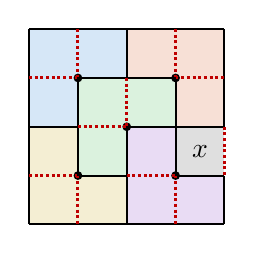
\begin{tikzpicture}[scale=0.62]
\fill[figA] (0,3) rectangle (1,4);
\fill[figA] (1,3) rectangle (2,4);
\fill[figA] (0,2) rectangle (1,3);
\fill[figB] (2,3) rectangle (3,4);
\fill[figB] (3,3) rectangle (4,4);
\fill[figB] (3,2) rectangle (4,3);
\fill[figC] (1,2) rectangle (2,3);
\fill[figC] (2,2) rectangle (3,3);
\fill[figC] (1,1) rectangle (2,2);
\fill[figD] (0,1) rectangle (1,2);
\fill[figD] (0,0) rectangle (1,1);
\fill[figD] (1,0) rectangle (2,1);
\fill[figE] (2,1) rectangle (3,2);
\fill[figE] (2,0) rectangle (3,1);
\fill[figE] (3,0) rectangle (4,1);
\fill[gray!25] (3,1) rectangle (4,2);
\node at (3.5,1.5) {$x$};
\fill[black] (1,3) circle (0.09);
\fill[black] (3,3) circle (0.09);
\fill[black] (2,2) circle (0.09);
\fill[black] (1,1) circle (0.09);
\fill[black] (3,1) circle (0.09);
\draw[ked] (0,4) -- (4,4);
\draw[ked] (1,3) -- (3,3);
\draw[ked] (0,2) -- (1,2);
\draw[ked] (2,2) -- (4,2);
\draw[ked] (1,1) -- (2,1);
\draw[ked] (3,1) -- (4,1);
\draw[ked] (0,0) -- (4,0);
\draw[ked] (0,4) -- (0,0);
\draw[ked] (1,3) -- (1,1);
\draw[ked] (2,4) -- (2,3);
\draw[ked] (2,2) -- (2,0);
\draw[ked] (3,3) -- (3,1);
\draw[ked] (4,4) -- (4,2);
\draw[ked] (4,1) -- (4,0);
\draw[gone] (0,3) -- (1,3);
\draw[gone] (3,3) -- (4,3);
\draw[gone] (1,2) -- (2,2);
\draw[gone] (0,1) -- (1,1);
\draw[gone] (2,1) -- (3,1);
\draw[gone] (1,4) -- (1,3);
\draw[gone] (3,4) -- (3,3);
\draw[gone] (2,3) -- (2,2);
\draw[gone] (4,2) -- (4,1);
\draw[gone] (1,1) -- (1,0);
\draw[gone] (3,1) -- (3,0);
\end{tikzpicture}
\caption{$4\times4$ 网格的刚性配置}
\label{fig:rigid44}
\end{figure}
\section{奇偶障碍定理}\label{sec:parity}

现在假设 $n,m\ge3$、$nm\equiv1\pmod3$，并且我们正在研究一个达到欧拉型下界的合法删除方案。根据引理~\ref{lem:rigid}，这样的方案必然具有刚性结构：只有一个小格 $x$ 没有被 L 形三格骨牌覆盖，而且整个网格只有一条被删除的边界边 $e_x$。下面要证明，这种结构会迫使网格的两个边长都是偶数。

证明的关键是先研究最上面的两行。我们需要知道：位于第一条内部水平线上的下型三格骨牌究竟能有多少个。

\begin{lemma}[顶部两行计数引理]\label{lem:band}
令
\[
\chi=
\begin{cases}
1,&e_x\in\{v(1,0),v(2,0),v(1,m),v(2,m)\},\\
0,&\text{否则}.
\end{cases}
\]
那么
\[
d_1\le\varepsilon_1+\chi-\varepsilon_2.
\]

该公式表明：
\begin{quote}
    如果小格 \(x\) 不在第一行，那么第一条内部水平线上一定没有下型三格骨牌，即 \(d_1=0\)。
\end{quote}

特别地，如果唯一未覆盖的小格 $x$ 不在第一行，那么 $d_1=0$。将网格上下翻转，可以得到对称结论：如果 $x$ 不在第 $n$ 行，那么 $u_{n-1}=0$。
\end{lemma}

\begin{proof}
我们只考察上边界和第二条内部水平线围成的所有矩形，也就是上下边分别位于水平线 $0$ 和水平线 $2$ 上的矩形。一个这样的矩形由两条竖直线 $j_1<j_2$ 确定。

如果竖直线 $j$ 上的边 $v(1,j)$ 或 $v(2,j)$ 被删除，就说这条竖直线在顶部两行中被\emph{破坏}。先数一数有多少条竖直线可能被这样破坏。

根据肘形结构：
\begin{itemize}
\item $v(1,j)$ 被删除，当且仅当水平线 $1$ 上、列 $j$ 处有一个上型三格骨牌中心；
\item $v(2,j)$ 被删除，当且仅当水平线 $1$ 上、列 $j$ 处有一个下型中心，或者水平线 $2$ 上、列 $j$ 处有一个上型中心。
\end{itemize}
因此，所有内部的、在顶部两行中被破坏的竖直线，其列编号一定属于以下两类位置：
\begin{itemize}
    \item 水平线 $1$ 上所有三格骨牌中心所在的列。
    \item 水平线 $2$ 上所有上型三格骨牌中心所在的列.
\end{itemize}

这样的内部竖直线至多有 $t_1+u_2$ 条。

对于 $j=0$ 和 $j=m$ 两条边界竖直线，它们只有在 $e_x$ 正好位于第一行或第二行时，才会在顶部两行中被破坏。因此，这两条边界竖直线中被破坏的条数至多为 $\chi$。如果记顶部两行中被破坏的竖直线总数为 $P$，那么
\[
P\le t_1+u_2+\chi.
\]
网格共有 $m+1$ 条竖直线，所以没有被破坏的竖直线条数 $U$ 满足
\[
U=(m+1)-P\ge m+1-t_1-u_2-\chi.
\]

接下来反过来考察这些没有被破坏的竖直线。任意取其中相邻的两条，记为 $j^{(s)}<j^{(s+1)}$。它们在第一行和第二行中的竖直边都保留。如果这两条竖直线之间，水平线 $0$ 和水平线 $2$ 上的边也全部保留，那么就会出现一个完整矩形。因此，在区间
\[
(j^{(s)},j^{(s+1)}]
\]
内，水平线 $0$ 或水平线 $2$ 至少有一条边必须被删除。

水平线 $0$ 是网格的最上边界。它上面唯一可能被删除的边就是 $e_x$；只有当 $x$ 位于第一行时才可能发生，所以这条线上的删除边数至多为 $\varepsilon_1$。另一方面，水平线 $2$ 上被删除的边恰好由中心位于水平线 $2$ 上的三格骨牌产生：每个这样的中心贡献一条被删除的水平边，总数为 $t_2$。由于 $n\ge3$，水平线 $2$ 不是网格边界线，不会受到 $e_x$ 的影响。

把所有没有被破坏的竖直线从左到右写成
\[
j^{(1)}<j^{(2)}<\cdots<j^{(U)}.
\]
相邻两条之间的区间 $(j^{(s)},j^{(s+1)}]$ 两两不重叠，而且每个区间都必须包含一条水平删除边。因此
\[
U-1\le t_2+\varepsilon_1.
\]
结合前面得到的
$U\ge m+1-t_1-u_2-\chi$，可得
\[
m\le t_1+u_2+t_2+\varepsilon_1+\chi.
\]
再利用第二行的行方程 \eqref{eq:row}：
\[
m=u_1+2d_1+2u_2+d_2+\varepsilon_2,
\]
以及 $t_1=u_1+d_1$、$t_2=u_2+d_2$，整理后得到
\[
d_1+\varepsilon_2\le\varepsilon_1+\chi,
\]
这就是所需不等式。

最后证明特别结论。若 $x$ 不在第一行，则 $\varepsilon_1=0$。如果此时 $\chi=0$，上面的不等式直接给出
$d_1\le-\varepsilon_2\le0$。如果 $\chi=1$，那么唯一被删除的边界边只能是第二行左端或右端的竖直边，即
$e_x\in\{v(2,0),v(2,m)\}$。这意味着 $x$ 位于第二行，所以 $\varepsilon_2=1$，从而
$d_1\le0+1-1=0$。由于 $d_1$ 是非负整数，必有 $d_1=0$。上下翻转网格即可得到另一端的结论。
\end{proof}

\begin{theorem}[奇偶障碍定理]\label{thm:parity}
设 $n,m\ge3$ 且 $nm\equiv1\pmod3$。如果
\[
S(n,m)=\ceil{2nm/3},
\]
那么 $n$ 和 $m$ 都是偶数。
\end{theorem}

\begin{proof}
取一个达到欧拉型下界的合法删除方案，并使用引理~\ref{lem:rigid} 中的记号。

先证明 $m$ 是偶数。分两种情况。

第一种情况：唯一未覆盖的小格 $x$ 不在第一行。由引理~\ref{lem:band}，有 $d_1=0$；同时 $\varepsilon_1=0$。将这些信息代入第一行方程 \eqref{eq:row}。因为网格顶部没有中心，$u_0=d_0=0$，所以方程化为
\[
m=2u_1.
\]
右边是偶数，因此 $m$ 是偶数。

第二种情况：$x$ 在第一行。由于 $n\ge3$，它不可能同时位于最后一行。由引理~\ref{lem:band} 的上下对称结论，有
$u_{n-1}=0$；而 $\varepsilon_n=0$。把这些信息代入最后一行的方程 \eqref{eq:row}，得到
\[
m=2d_{n-1}.
\]
所以 $m$ 仍然是偶数。

至此，我们已经证明 $m$ 必须是偶数。现在把整个网格转置，也就是交换行和列，得到一个 $m\times n$ 网格。转置不会改变矩形是否存在，也不会改变需要删除的边数，因此同样的论证可以用于这个转置后的网格。由此可知 $n$ 也必须是偶数。
\end{proof}

\begin{corollary}\label{cor:families}
下面四组下界都可以由人工证明得到；结合第~\ref{sec:exact} 节给出的上界，它们实际上都是等式：
\begin{enumerate}
\item $S(5,3k+2)\ge10k+8$，其中 $k\ge0$；
\item $S(7,3k+1)\ge14k+6$，其中 $k\ge1$；
\item 当 $m\equiv5\pmod6$ 时，$S(8,m)\ge(16m+4)/3$；
\item 当 $m\equiv1\pmod6$ 时，$S(4,m)\ge\ceil{8m/3}+1$。
\end{enumerate}
\end{corollary}

\begin{proof}
在上述四种情形中，都有 $nm\equiv1\pmod3$，但 $n,m$ 不可能同时为偶数：前两种情形中 $n$ 是奇数，后两种情形中 $m$ 是奇数。因此，根据定理~\ref{thm:parity}，欧拉型下界不可能取等号。由于 $S(n,m)$ 是整数，它至少要比欧拉型下界大 $1$，得到所列结论。
\end{proof}


\section{高度 $4$ 到 $8$ 的精确值}\label{sec:exact}

下面列出 $n=4,5,6,7,8$ 时的全部精确公式。每个定理中的下界都注明了证明来源。上界的证明方式稍有不同：在有限多个小宽度上，程序通过动态规划找到具体的删除边集合；我们再用一个独立的穷举程序，把所有可能的矩形逐一检查，确认每个矩形至少有一条边被删除。对于更大的 $m$，则利用引理~\ref{lem:cert} 中已经证明的状态重复规律，把有限计算结果推广到所有宽度。

\begin{theorem}[$n=4$]\label{thm:n4}
$S(4,1)=4$；对所有 $m\ge2$，
\[
S(4,m)=\ceil{30m/11}.
\]
\end{theorem}

下面的命题给出这个公式的下界。读者可以把其中的函数 $\Psi$ 理解为给每个扫描状态分配一个非负的“势能值”。它的变化量能够控制每增加一列时必须删除多少条边。把每一步的不等式加起来，势能项会相互抵消，只留下总删除边数的下界。

\begin{proposition}[高度 $4$ 的势函数验证表]\label{prop:psi}
存在一个函数
\[
\Psi:\mathcal R\longrightarrow\{0,1,\ldots,46\},
\]
其中 $\mathcal R$ 是高度 $n=4$ 的扫描过程中所有可能到达的 $522$ 个状态（完整数据保存在 \texttt{psi4.json} 中），并且满足以下三组条件：

\emph{(C1)} 对每个状态 $s$，都有 $\Psi(s)\ge0$。

\emph{(C2)} 对每一种初始选择 $V_0$，初始状态满足
\[
\Psi(\mathrm{live}_0)\le
11\times(\text{第 }0\text{ 条竖直线上的删除边数}).
\]

\emph{(C3)} 对每个可达状态 $s$，以及从它出发的每一种合法列选择 $(H,V)$，若新状态为 $s'$，则
\[
\Psi(s')\le
\Psi(s)+11\times(\text{本列删除边数})-30.
\]

这三组条件都只涉及有限多个状态和转移。计算程序已经逐项检查了其中每一条不等式，全部成立。由此可以推出，对所有 $m\ge1$，
\[
S(4,m)\ge\frac{30m}{11},
\]
由于 $S(4,m)$ 是整数，进一步得到
$S(4,m)\ge\ceil{30m/11}$。
\end{proposition}

\begin{proof}[证明（假设 C1--C3 已逐项验证）]
任取一个合法删除方案。根据引理~\ref{lem:exact}，它对应一条状态轨迹
$s_0,s_1,\ldots,s_m$。设整个方案一共删除了 $K$ 条边。把初始条件 (C2) 和每一步的条件 (C3) 相加，得到
\[
11K
\ge
\Psi(s_0)+\sum_{i=1}^{m}
\bigl(30+\Psi(s_i)-\Psi(s_{i-1})\bigr).
\]
右边的势函数项会逐项抵消，只剩下
\[
11K\ge30m+\Psi(s_m).
\]
再由 (C1) 知道 $\Psi(s_m)\ge0$，因此
\[
11K\ge30m.
\]
这对任意合法删除方案都成立，所以最少删除边数也满足
$S(4,m)\ge30m/11$。
\end{proof}

\begin{remark}
势函数下界还可以从最优方案的局部结构中得到解释。考虑一个长度为 $11$ 列的周期区域。假设其中有 $t$ 个 L 形三格骨牌区域和 $q$ 个非矩形的四小格区域。每个三格骨牌覆盖 $3$ 个小格、对应 $2$ 条被删除的内部边；每个这样的四小格区域覆盖 $4$ 个小格、对应 $3$ 条被删除的内部边。因为高度为 $4$，这 $11$ 列一共包含 $44$ 个小格，并且要删除 $30$ 条边，所以
\[
3t+4q=44,\qquad 2t+3q=30.
\]
解得 $t=12$、$q=2$。也就是说，每 $11$ 列中必须出现 $2$ 个这样的四小格区域。这正是高度 $4$ 的删除密度高于 $8/3$ 的组合原因。势函数 $\Psi$ 则把这种额外的删除需求转化成了一个可以逐步累加的数学不等式。
\end{remark}

\begin{theorem}[$n=5$：补全 \cite{NT25} 中的两个缺口]\label{thm:n5}
$S(5,1)=5$；对 $m\ge2$，
\[
S(5,m)=\begin{cases}
\dfrac{10m}{3}+1, & m\equiv0\pmod3\quad(\text{下界由定理~\ref{thm:euler} 给出；亦见 \cite{NT25}}),\\[4pt]
\dfrac{10m+2}{3}, & m\equiv1\pmod3\quad(\text{下界由定理~\ref{thm:euler} 给出}),\\[4pt]
\dfrac{10m+4}{3}, & m\equiv2\pmod3\quad(\text{下界由系~\ref{cor:families}(i) 给出}).
\end{cases}
\]
特别地，当 $m\equiv1\pmod3$ 时，\cite{NT25} 原来的下界是正确的，但上界可以减少 $1$；当 $m\equiv2\pmod3$ 时，原来的上界是正确的，但下界需要增加 $1$。
\end{theorem}

\begin{theorem}[$n=6$]\label{thm:n6}
$S(6,1)=6$；对所有 $m\ge2$，
\[
S(6,m)=4m+1.
\]
下界由定理~\ref{thm:euler} 直接得到，因为 $3\mid6m$ 对所有整数 $m$ 都成立。
\end{theorem}

\begin{theorem}[$n=7$]\label{thm:n7}
$S(7,1)=7$、$S(7,2)=11$；对 $m\ge3$，
\[
S(7,m)=\begin{cases}
\dfrac{14m}{3}+1, & m\equiv0\pmod3\quad(\text{下界由定理~\ref{thm:euler} 给出}),\\[4pt]
\dfrac{14m+4}{3}, & m\equiv1\pmod3\quad(\text{下界由系~\ref{cor:families}(ii) 给出}),\\[4pt]
\dfrac{14m+2}{3}, & m\equiv2\pmod3\quad(\text{下界由定理~\ref{thm:euler} 给出}).
\end{cases}
\]
\end{theorem}

\begin{theorem}[$n=8$]\label{thm:n8}
$S(8,1)=8$、$S(8,2)=12$；对 $m\ge3$，
\[
S(8,m)=\begin{cases}
\dfrac{16m}{3}+1, & m\equiv0\pmod3,\\[4pt]
\dfrac{16m+2}{3}, & m\equiv1\pmod3,\\[4pt]
\dfrac{16m+1}{3}+[\,m\text{ 为奇数}\,],
& m\equiv2\pmod3\quad(\text{奇数情形的下界由系~\ref{cor:families}(iii) 给出}).
\end{cases}
\]
\end{theorem}

\begin{remark}
定理~\ref{thm:n8} 中 $m\equiv2\pmod3$ 的情形还要进一步区分 $m$ 的奇偶性。当 $m$ 为偶数（例如 $m=8,14,20,\ldots$）时，欧拉型下界能够取到；当 $m$ 为奇数时，奇偶障碍定理说明欧拉型下界不能取到，所以答案要再增加 $1$。特别地，$8\times8$ 的情形就是 Golomb 构造所涉及的经典例子；关于残缺棋盘的三格骨牌铺砌，可参见 \cite{CJ86}。

这说明，不能只根据 $nm$ 除以 $3$ 的余数来决定
\[
\varepsilon(n,m):=S(n,m)-\ceil{2nm/3}.
\]
真正的情况还取决于是否存在达到欧拉型下界的刚性配置。综合本文结果（$m\ge3$，忽略少数小尺寸例外），有以下规律：当 $nm\equiv0\pmod3$ 时，$\varepsilon=1$；当 $nm\equiv2\pmod3$ 时，$\varepsilon=0$；当 $nm\equiv1\pmod3$ 且 $n,m$ 不全为偶数时，$\varepsilon=1$。对于 $n=8$ 且 $m\ge8$ 为偶数的情形，计算结果显示 $\varepsilon=0$。
\end{remark}

下面的表格汇总了 $m\le14$ 时的计算结果。对于更大的 $m$，可以直接使用上面各定理中的公式。
\begin{center}\small
\begin{tabular}{c|cccccccccccccc}
\toprule
$m$ & 1&2&3&4&5&6&7&8&9&10&11&12&13&14\\
\midrule
$S(4,m)$ & 4&6&9&11&14&17&$20$&22&25&$28$&30&33&$36$&$39$\\
$S(5,m)$ & 5&8&11&14&18&21&24&28&31&34&38&41&44&48\\
$S(6,m)$ & 6&9&13&17&21&25&29&33&37&41&45&49&53&57\\
$S(7,m)$ & 7&11&15&20&24&29&34&38&43&48&52&57&62&66\\
$S(8,m)$ & 8&12&17&22&28&33&38&43&49&54&60&65&70&75\\
\bottomrule
\end{tabular}
\end{center}


\begin{figure}[htbp]\centering
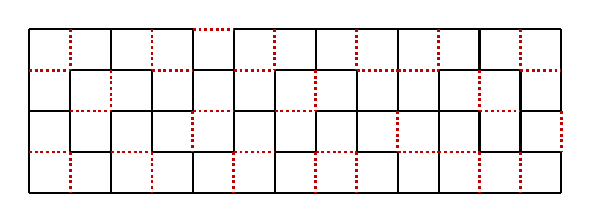
\begin{tikzpicture}[scale=0.52]
\draw[ked] (0,4) -- (4,4);
\draw[ked] (5,4) -- (13,4);
\draw[ked] (1,3) -- (3,3);
\draw[ked] (4,3) -- (5,3);
\draw[ked] (6,3) -- (8,3);
\draw[ked] (10,3) -- (12,3);
\draw[ked] (0,2) -- (1,2);
\draw[ked] (2,2) -- (4,2);
\draw[ked] (5,2) -- (6,2);
\draw[ked] (7,2) -- (11,2);
\draw[ked] (12,2) -- (13,2);
\draw[ked] (1,1) -- (2,1);
\draw[ked] (3,1) -- (5,1);
\draw[ked] (6,1) -- (7,1);
\draw[ked] (8,1) -- (9,1);
\draw[ked] (11,1) -- (13,1);
\draw[ked] (0,0) -- (13,0);
\draw[ked] (0,4) -- (0,0);
\draw[ked] (1,3) -- (1,1);
\draw[ked] (2,4) -- (2,3);
\draw[ked] (2,2) -- (2,0);
\draw[ked] (3,3) -- (3,1);
\draw[ked] (4,4) -- (4,2);
\draw[ked] (4,1) -- (4,0);
\draw[ked] (5,4) -- (5,1);
\draw[ked] (6,3) -- (6,0);
\draw[ked] (7,4) -- (7,3);
\draw[ked] (7,2) -- (7,1);
\draw[ked] (8,3) -- (8,1);
\draw[ked] (9,4) -- (9,2);
\draw[ked] (9,1) -- (9,0);
\draw[ked] (10,3) -- (10,0);
\draw[ked] (11,4) -- (11,3);
\draw[ked] (11,2) -- (11,1);
\draw[ked] (12,3) -- (12,1);
\draw[ked] (13,4) -- (13,2);
\draw[ked] (13,1) -- (13,0);
\draw[gone] (4,4) -- (5,4);
\draw[gone] (0,3) -- (1,3);
\draw[gone] (3,3) -- (4,3);
\draw[gone] (5,3) -- (6,3);
\draw[gone] (8,3) -- (9,3);
\draw[gone] (9,3) -- (10,3);
\draw[gone] (12,3) -- (13,3);
\draw[gone] (1,2) -- (2,2);
\draw[gone] (4,2) -- (5,2);
\draw[gone] (6,2) -- (7,2);
\draw[gone] (11,2) -- (12,2);
\draw[gone] (0,1) -- (1,1);
\draw[gone] (2,1) -- (3,1);
\draw[gone] (5,1) -- (6,1);
\draw[gone] (7,1) -- (8,1);
\draw[gone] (9,1) -- (10,1);
\draw[gone] (10,1) -- (11,1);
\draw[gone] (1,4) -- (1,3);
\draw[gone] (3,4) -- (3,3);
\draw[gone] (6,4) -- (6,3);
\draw[gone] (8,4) -- (8,3);
\draw[gone] (10,4) -- (10,3);
\draw[gone] (12,4) -- (12,3);
\draw[gone] (2,3) -- (2,2);
\draw[gone] (7,3) -- (7,2);
\draw[gone] (11,3) -- (11,2);
\draw[gone] (4,2) -- (4,1);
\draw[gone] (9,2) -- (9,1);
\draw[gone] (13,2) -- (13,1);
\draw[gone] (1,1) -- (1,0);
\draw[gone] (3,1) -- (3,0);
\draw[gone] (5,1) -- (5,0);
\draw[gone] (7,1) -- (7,0);
\draw[gone] (8,1) -- (8,0);
\draw[gone] (11,1) -- (11,0);
\draw[gone] (12,1) -- (12,0);
\end{tikzpicture}
\caption{$S(4,13)=36=\ceil{390/11}$ 的一个最优删除方案。它比欧拉型下界 $35$ 多删除一条边。红色虚线表示被删除的边；该方案已经由独立的穷举程序逐个检查所有矩形，确认是合法的。}
\label{fig:sol413}
\end{figure}

\begin{figure}[htbp]\centering
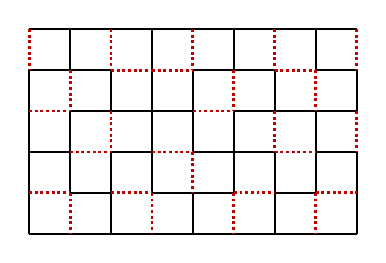
\begin{tikzpicture}[scale=0.52]
\draw[ked] (0,5) -- (8,5);
\draw[ked] (0,4) -- (2,4);
\draw[ked] (4,4) -- (6,4);
\draw[ked] (7,4) -- (8,4);
\draw[ked] (1,3) -- (4,3);
\draw[ked] (5,3) -- (8,3);
\draw[ked] (0,2) -- (1,2);
\draw[ked] (2,2) -- (3,2);
\draw[ked] (4,2) -- (6,2);
\draw[ked] (7,2) -- (8,2);
\draw[ked] (1,1) -- (2,1);
\draw[ked] (3,1) -- (5,1);
\draw[ked] (6,1) -- (7,1);
\draw[ked] (0,0) -- (8,0);
\draw[ked] (0,4) -- (0,0);
\draw[ked] (1,5) -- (1,4);
\draw[ked] (1,3) -- (1,1);
\draw[ked] (2,4) -- (2,3);
\draw[ked] (2,2) -- (2,0);
\draw[ked] (3,5) -- (3,1);
\draw[ked] (4,4) -- (4,2);
\draw[ked] (4,1) -- (4,0);
\draw[ked] (5,5) -- (5,4);
\draw[ked] (5,3) -- (5,1);
\draw[ked] (6,4) -- (6,3);
\draw[ked] (6,2) -- (6,0);
\draw[ked] (7,5) -- (7,4);
\draw[ked] (7,3) -- (7,1);
\draw[ked] (8,4) -- (8,3);
\draw[ked] (8,2) -- (8,0);
\draw[gone] (2,4) -- (3,4);
\draw[gone] (3,4) -- (4,4);
\draw[gone] (6,4) -- (7,4);
\draw[gone] (0,3) -- (1,3);
\draw[gone] (4,3) -- (5,3);
\draw[gone] (1,2) -- (2,2);
\draw[gone] (3,2) -- (4,2);
\draw[gone] (6,2) -- (7,2);
\draw[gone] (0,1) -- (1,1);
\draw[gone] (2,1) -- (3,1);
\draw[gone] (5,1) -- (6,1);
\draw[gone] (7,1) -- (8,1);
\draw[gone] (0,5) -- (0,4);
\draw[gone] (2,5) -- (2,4);
\draw[gone] (4,5) -- (4,4);
\draw[gone] (6,5) -- (6,4);
\draw[gone] (8,5) -- (8,4);
\draw[gone] (1,4) -- (1,3);
\draw[gone] (5,4) -- (5,3);
\draw[gone] (7,4) -- (7,3);
\draw[gone] (2,3) -- (2,2);
\draw[gone] (6,3) -- (6,2);
\draw[gone] (8,3) -- (8,2);
\draw[gone] (4,2) -- (4,1);
\draw[gone] (1,1) -- (1,0);
\draw[gone] (3,1) -- (3,0);
\draw[gone] (5,1) -- (5,0);
\draw[gone] (7,1) -- (7,0);
\end{tikzpicture}
\caption{$S(5,8)=28=10\cdot2+8$ 的一个最优删除方案。这给出了 $m\equiv2\pmod3$ 时的上界；相应下界由系~\ref{cor:families}(i) 的人工证明得到。}
\label{fig:sol58}
\end{figure}
\section{分层拼接、一般上界与渐近密度}\label{sec:stack}

前面已经确定了高度 $3,4,5$ 的精确值。现在利用这些较低高度的结果，构造更高网格的删除方案。基本想法是把一个高网格从上到下分成若干条带，分别在每条带中使用已经知道的删除方案，再把它们拼在一起。

不过，这里有一个需要特别注意的问题：即使每一条带内部都没有矩形，拼接之后仍可能出现一个矩形，它的上边在上层、下边在下层，左右两条边则穿过不同的条带。为了排除这种跨层矩形，我们需要给除最下层以外的每条带增加一个接口条件。

对高度为 $h$ 的条带网格，定义接口条件 $(*)$ 如下：不存在一条水平线
$i\in\{0,\ldots,h-1\}$ 和两条竖直线 $j_1<j_2$，使得在这两条竖直线上，从第 $i+1$ 行一直到条带底部的竖直边都保留，同时水平线 $i$ 上从 $j_1$ 到 $j_2$ 的边也全部保留。直观地说，接口条件禁止出现这样一种情况：某条带中有一个矩形的上边和两条向下延伸的竖边都完整保留，以至于它们可能与下方条带中的边拼成一个更大的矩形。

记 $S^*(h,m)$ 为高度 $h$、宽度 $m$ 的条带中，在删除方案合法且满足接口条件 $(*)$ 的前提下，所需删除的最少边数。因此显然有
$S(h,m)\le S^*(h,m)$。

\begin{lemma}[分层拼接引理]\label{lem:stack}
把高度为 $n$ 的网格从上到下分成 $t$ 条带，各条带高度分别为
$n_1,\ldots,n_t$，其中 $n=n_1+\cdots+n_t$。如果前 $t-1$ 条带分别采用满足接口条件 $(*)$ 的合法删除方案，最下方一条带采用任意合法删除方案，那么把这些删除方案合并起来，得到的就是整个 $n\times m$ 网格的合法删除方案。因此
\[
S\left(\sum_{i=1}^t n_i,m\right)
\le
\sum_{i=1}^{t-1}S^*(n_i,m)+S(n_t,m).
\]
\end{lemma}

\begin{proof}
只要检查拼接后的网格中是否可能出现跨越不同条带的矩形。

如果一个矩形完全位于某一条带内，那么它已经被该条带的合法删除方案破坏。即使矩形的一条边恰好落在条带的上边界或下边界上，也仍然属于这一类。

因此，只需考虑真正跨越条带边界的矩形。取这个矩形最上方的一条水平边。它必然位于某条非最下层条带 $A$ 的内部水平线 $i$ 上，或者位于该条带的上边界线上。若它位于 $A$ 的下边界线上，那么矩形实际上从下一条带开始，应把注意力转移到下方条带；所以我们只需考虑 $0\le i\le n_A-1$ 的情况。

如果这个矩形没有被破坏，那么它的左右两条竖边在条带 $A$ 中都必须从水平线 $i$ 一直保留到 $A$ 的底部；同时，它的上边也必须在整个区间 $(j_1,j_2]$ 内完整保留。这恰好违反条带 $A$ 的接口条件 $(*)$。因此，任何跨层矩形都不可能存在，拼接后的删除方案合法。
\end{proof}

\begin{fact}\label{fact:star}
对高度 $3,4,5$，接口条件 $(*)$ 不会增加最少删除边数。更具体地说，有限范围内的计算给出
\[
S^*(3,m)=S(3,m),\quad
S^*(4,m)=S(4,m),\quad
S^*(5,m)=S(5,m).
\]
再利用引理~\ref{lem:cert} 的状态重复规律，可以把这些等式从有限范围推广到所有 $m$。
\end{fact}

\begin{theorem}[一般上界；修补并推广 \cite{NT25} 定理 3]\label{thm:general}
记
\[
c(m)=S(5,m)-\frac{10m}{3}
\in\left\{\frac23,1,\frac43\right\}
\qquad(m\ge2).
\]
那么对所有 $m\ge2$，有
\[
S(n,m)\le
\begin{cases}
\dfrac{2nm}{3}+\dfrac n3,
& n\equiv0\pmod3,\ n\ge3,\\[4pt]
\dfrac{2nm}{3}+\dfrac{n-5}{3}+c(m)
\le\dfrac{2nm}{3}+\dfrac{n-1}{3},
& n\equiv2\pmod3,\ n\ge5,\\[4pt]
\dfrac{2nm}{3}+\dfrac{n-10}{3}+2c(m)
\le\dfrac{2nm}{3}+\dfrac{n-2}{3},
& n\equiv1\pmod3,\ n\ge10,\\[4pt]
(2m+1)+\ceil{30m/11},
& n=7.
\end{cases}
\]
\end{theorem}

\begin{proof}
根据 $n$ 除以 $3$ 的余数，把高度为 $n$ 的网格分成高度为 $3$ 和 $5$ 的条带；当 $n=7$ 时，分成高度为 $3$ 和 $4$ 的两条带。除了最下方的条带以外，其他条带都采用事实~\ref{fact:star} 中满足接口条件、且删除边数最少的方案；最下方条带只需要采用普通的最优删除方案。然后应用分层拼接引理~\ref{lem:stack}，再代入定理~\ref{thm:n4}、定理~\ref{thm:n5} 和已知公式 $S(3,m)=2m+1$，即可得到上述各个上界。
\end{proof}

\begin{remark}
\cite{NT25} 定理 3 的证明直接把若干条带的删除边数相加，但如果不额外说明接口条件，就不能排除跨越条带的矩形。分层拼接引理补上了这一环节，而事实~\ref{fact:star} 又说明：在高度 $3,4,5$ 的情形下，增加接口条件并不会增加删除边数。

此外，本定理去掉了 \cite{NT25} 原来要求的 $m\ge n\ge8$ 限制。对于 $n\equiv0\pmod3$ 的情形，得到的加法常数与原结果相同；其他情形的上界更小。结合定理~\ref{thm:euler}，当 $3\mid n$ 时有
\[
\frac{2nm}{3}+1\le S(n,m)\le\frac{2nm}{3}+\frac n3.
\]
因此，加在主项 $2nm/3$ 后面的常数位于 $[1,n/3]$ 之间。定理~\ref{thm:n6} 还表明，当 $n=6$ 时取到这个区间的下端点。
\end{remark}

\begin{theorem}[渐近密度]\label{thm:density}
极限
\[
\delta(n):=\lim_{m\to\infty}\frac{S(n,m)}m
\]
存在，并且
\[
\delta(1)=1,\quad
\delta(2)=\frac32,\quad
\delta(3)=2,\quad
\delta(4)=\frac{30}{11},\quad
\delta(n)=\frac{2n}{3}\quad(n\ge5).
\]
\end{theorem}

\begin{proof}
当 $n\le8$ 时，直接由前面得到的精确公式计算极限即可。当 $n\ge9$ 时，下界由定理~\ref{thm:euler} 给出，上界由定理~\ref{thm:general} 给出。对 $n\ne7$，一般上界中关于 $m$ 的主项斜率都是 $2n/3$，所以上下界除以 $m$ 后在 $m\to\infty$ 时趋于同一个数 $2n/3$。因此极限存在，并且等于 $2n/3$。
\end{proof}
\section{计算实现、独立检查与复现}\label{sec:comp}

\textbf{扫描程序如何运行。}
引理~\ref{lem:exact}--\ref{lem:cert} 中的扫描算法使用 Python 实现，主要程序为 \texttt{rect.py}。程序包括状态支配剪枝，并使用 $\mathrm{live}\cap K_H$ 作为展开缓存的键；\texttt{drive.py} 用于在较大规模计算中保存检查点并从检查点继续运行。对 $n\le8$ 的计算都可以在数分钟内完成，并输出可以逐项检查的状态数据。

程序还会回溯出达到最优值的具体删除边集合。为了避免只依赖同一个程序给出的结果，我们另写了一个独立的穷举验证程序：对每个候选删除方案，它逐一枚举
\[
\binom{n+1}{2}\binom{m+1}{2}
\]
个可能的矩形，也就是枚举所有水平线对和竖直线对，并检查每个矩形是否至少有一条边被删除。只有通过这项检查的方案，才被作为合法上界使用。

\textbf{独立交叉检查。}
我们还进行了以下几类相互独立的检查：

\begin{enumerate}
\item 程序逐项重现 \cite{NT25} 中的 $S(1,m),S(2,m),S(3,m)$（$m\le12$）、$S(4,4)=11$、$S(5,3k)=10k+1$，以及 Golomb 的数值 $S(8,8)=43$。
\item 检查转置一致性 $S(a,b)=S(b,a)$。在所有重叠的计算范围内，这个关系都成立。例如，以下等式均得到验证：
\[
S(4,5)=S(5,4)=14,\qquad
S(7,k)=S(k,7)\ (k\le6),\qquad
S(8,k)=S(k,8)\ (k\le7).
\]
\item 使用完全独立的整数规划程序 CBC（代码文件为 \texttt{ilp.py}）复核部分数值：检查了 $S(4,m)$ 在
$m\in\{2,3,5,6,7,8,9\}$ 时的值，以及 $S(5,m)$ 在
$m\in\{5,7,8\}$ 时的值，结果全部一致。
\item 使用 \texttt{gen\_all.py} 从展示的删除方案中重新构造平面区域，并逐项检查引理~\ref{lem:rigid}--\ref{lem:band} 中涉及的结构性质，包括图~\ref{fig:rigid44} 的例子。
\item 使用 \texttt{potential.py} 检查命题~\ref{prop:psi} 中的 C1--C3 条件。程序检查了 $522$ 个状态以及它们的全部合法转移，没有发现任何一条不等式不成立。
\end{enumerate}

\textbf{复现所需文件。}
完整计算使用以下文件：
\begin{itemize}
\item \texttt{rect.py}：扫描算法、最优方案回溯和合法性验证；
\item \texttt{drive.py}：较大规模计算的检查点保存与续算；
\item \texttt{ilp.py}：独立的整数规划复核程序；
\item \texttt{potential.py} 和 \texttt{psi4.json}：生成并保存高度 $4$ 的势函数数据；
\item \texttt{gen\_all.py}：检查刚性结构并生成图形。
\end{itemize}
所有计算都是确定性的。在普通桌面计算机上，完整运行全部程序预计可以在一小时内完成。需要强调的是，程序只负责产生和核验有限范围内的数据；“对所有 $m$ 成立”的结论还需要引理~\ref{lem:cert} 所证明的状态重复规律，不能仅凭有限次运行直接得出。

\section{结论、勘误与后续问题}\label{sec:open}

本文对 \cite{NT25} 有三点补充说明：

\begin{enumerate}
\item 该文定理 1 中“下界再加 $1$”的条件应为 $3\mid nm$，而不只是 $n\equiv0\pmod3$；见注~\ref{rem:errata}。
\item 该文定理 3 直接把不同条带的删除方案相加时，需要补充接口条件，以排除跨越条带的矩形。本文的引理~\ref{lem:stack} 给出了完整论证，而事实~\ref{fact:star} 说明对高度 $3,4,5$ 来说，这个接口条件不增加最优删除边数。
\item 该文定理 5 中，当 $m\equiv1\pmod3$ 时，上界构造还可以少删除一条边；见定理~\ref{thm:n5}。
\end{enumerate}

本文还留下了若干值得继续研究的问题。

\begin{conjecture}[两个边长均为偶数时的充分性]\label{conj:even}
存在一个常数 $N$，使得只要
\[
\min(n,m)\ge N,\qquad nm\equiv1\pmod3,
\]
并且 $n,m$ 都是偶数，就有
\[
S(n,m)=\ceil{2nm/3}.
\]
目前的计算结果支持 $N\le8$：当 $n=8$、$m\equiv2\pmod6$ 且 $m\ge8$ 时，欧拉型下界都能够取到。
\end{conjecture}

其他后续方向包括：

\begin{enumerate}
\item \textbf{确定 $n\ge9$ 时的精确值。}本文的扫描方法可以继续用于更高的网格。下一步可以先研究 $n=9,10$，直接检验猜想~\ref{conj:even}，以及另一个猜测：当 $3\mid n$ 且 $m$ 足够大时，是否总有
$S(n,m)=2nm/3+1$。目前 $n=6$ 已经满足这个等式。
\item \textbf{寻找高度 $4$ 下界的纯组合证明。}命题~\ref{prop:psi} 通过势函数表证明了 $S(4,m)\ge30m/11$。如果能给势函数 $\Psi$ 找到一个直接的组合解释，例如类似放电法的计数规则，就有希望把这部分证明完全改写为人工证明。
\item \textbf{进一步确定正方形网格的加法项。}可以继续研究 $S(n,n)$ 中主项之外的加法项，并与 \cite{NT25} 定理 6 对照。
\item \textbf{完整刻画刚性配置何时存在。}当 $nm\equiv1\pmod3$ 且 $n,m$ 都是偶数时，奇偶障碍定理不再排除欧拉型下界达到等号的可能性。但这并不意味着取等号一定成立。需要进一步确定
$\varepsilon(n,m)=S(n,m)-\ceil{2nm/3}$
在这些情形下的具体取值。
\end{enumerate}
\begin{thebibliography}{9}
\bibitem{NT25} E.~Niu, Z.~Tang, On the rectangle eliminating number of grid graphs, in: \emph{Theory and Applications of Models of Computation (TAMC 2025)}, LNCS 16084, Springer, 2025, pp.~207--220（及它的期刊扩充版，投稿于 \emph{Theoretical Computer Science}, 2026）.
\bibitem{Golomb54} S.~W.~Golomb, Checker boards and polyominoes, \emph{Amer. Math. Monthly} \textbf{61} (1954) 675--682.
\bibitem{CJ86} I-P.~Chu, R.~Johnsonbaugh, Tiling deficient boards with trominoes, \emph{Math. Mag.} \textbf{59} (1986) 34--40.
\end{thebibliography}

\end{document}